\documentclass[12pt,center]{beamer}

%%%%%%%%%%% Lo que viene  a continuacion es el tipo de presentacion que quieres, 
% las presentaciones se llaman con nombres de ciudades puedes cambiarlas y tomar
%%%%%%%%la que mas te guste.
\mode<presentation> {
  %\usetheme{Frankfurt}
  %\usetheme{Warsaw}
  %\usetheme{Darmstadt}
   %\usetheme{Dresden}
  \usetheme{Singapore}
  %\usetheme{Bergen}
  %\usetheme{Boadilla}
  %\usetheme{BerKeley}
  \setbeamercovered{transparent}
  %\setbeamertemplate{background canvas}[vertical shading][bottom=red!20,top=yellow!30]
%   \setbeamertemplate{headline}{}
%%%%%%%%%%%%%%%%%%%%%%%%%%%%%%%%%%
%%%%%%% aqui vienen los colores

  %\usecolortheme{crane}
  %\usecolortheme{seahorse}
  \usecolortheme{whale}
  %\usecolortheme{rose}
  %\usecolortheme{orchid}
} \usepackage{alltt}



%%%%%%%los paquetes. 
\usepackage{amssymb,amsmath,latexsym}
%\usepackage[mathcal]{euscript}
%\usepackage[polish]{babel}
%\usepackage{dsfont}
%\usepackage[normalem]{ulem}
\usepackage{enumerate}
%\usepackage[all,2cell,dvips]{xy} \UseAllTwocells \SilentMatrices

\usepackage{verbatim}
\usepackage{float}

\usepackage[utf8x]{inputenc}
\usepackage{url}
\usepackage{makeidx}
\usepackage[procnames]{listings}
\usepackage{color}
\usepackage{graphicx} % graficos
\usepackage{subfig}
\usepackage{tabularx}
%\usepackage{subcaption}
\captionsetup{compatibility=false}
\usepackage[export]{adjustbox}
\usepackage[spanish]{babel}
\usepackage{mathtools}
\usepackage{svg}
\title{Transferencia de Estilo en Fotografias mediante Redes Neuronales Convolucionales}
%
%
\author{Ariel Wolfmann}

%
\institute{Facultad de Matemática, Astronomía, Física y Computación\\
	  Universidad Nacional de Córdoba}

\date{28 de Julio, 2017}


\begin{document}
%%%%%%%%%%%%%%%%%%%%%%%%%%%PAGINA DEL TITULO
\begin{frame}
  \titlepage
\end{frame}

%%%%%%%%%%%%%%%%%  tODO LO QUE QUIERAS PONER EN LOS FRAMES.
\begin{frame}
  \frametitle{Agenda}
  \tableofcontents[pausesections]
\end{frame}
  %  \tableofcontents[pausesections]
%   %You might wish to add the option [pausesections]


%%%%%%%%%%%%%%%%%%%%%%%% EFDs & Algebraic Functions %%%%%%%%%%%%%%%%%%%%%%%%%%%%
\section{Introducción}
\begin{frame}
  \frametitle{Contexto}
  Aplicaciones de efectos en fotografias:
    \begin{figure}[H]
      \begin{center}
	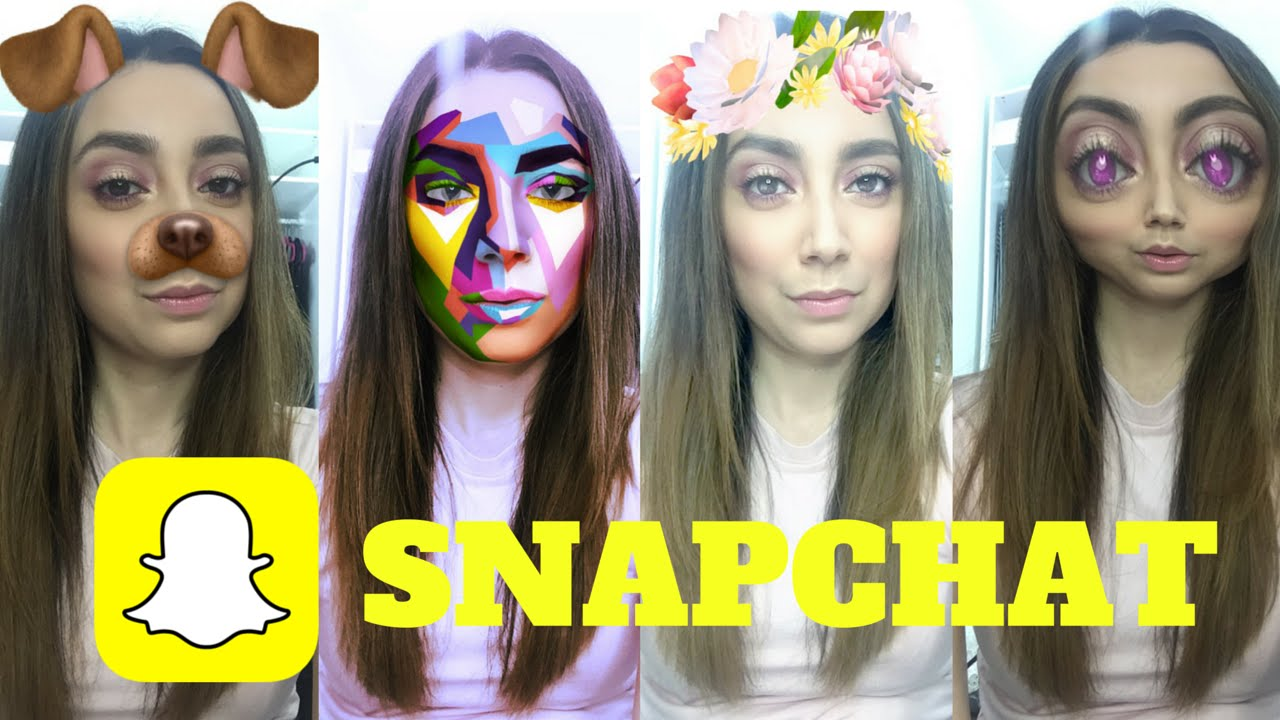
\includegraphics[width=0.8\linewidth]{./img/filtro_snapchat.jpg}
      \end{center}
      %\caption{Ejemplos de síntesis de texturas utilizando Redes Neuronales Convolucionales}
      %\label{fig:textures}
    \end{figure}
\end{frame}	

\begin{frame}
  \frametitle{Como se representa una imágen}
  Arreglo de píxeles ordenados
    \begin{figure}[H]
      \begin{center}
	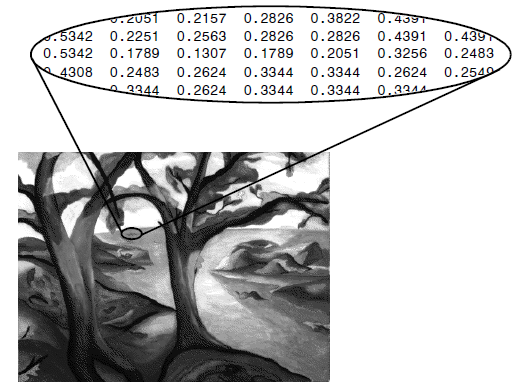
\includegraphics[width=0.8\linewidth]{./img/image_pixel.png}
      \end{center}
    \end{figure}
\end{frame}
  
\begin{frame}
  \frametitle{Aprendizaje automatico en vision por computadoras}
  \begin{itemize}
    \item \textbf{Vision por computadoras} (Computer Vision): Comprensión de alto nivel sobre imágenes digitales, busca automatizar tareas del sistema visual humano.
    \item \textbf{Aprendizaje automático} (Machine Learning): Algortimos que otorgan a las computadoras la habilidad de aprender y hacer predicciones sobre los datos de entrada. 
  \end{itemize}

  
    \begin{figure}[H]
      \begin{center}
	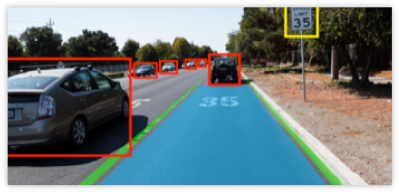
\includegraphics[width=0.8\linewidth]{./img/nvidia_car_detection.png}
      \end{center}
      \caption{Vehiculos autónomos}
      %\label{fig:textures}
    \end{figure}    
\end{frame}
  
\begin{frame}
  \frametitle{Transferencia de estilo}
  A partir de una imagen de contenido y una imagen de estilo se genera una nueva imagen que combina ambos.
  \begin{figure}[h]
    \begin{center}
      \subfloat[Imagen de Estilo]{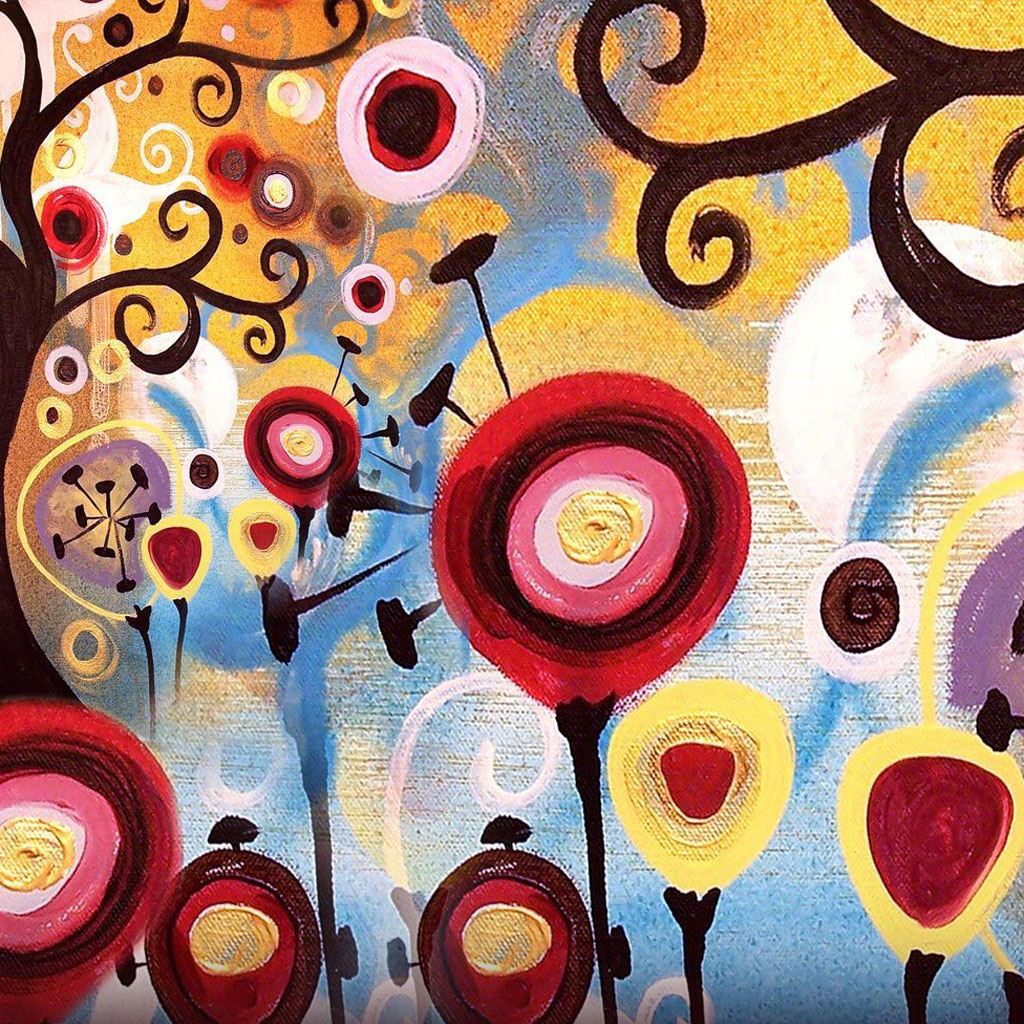
\includegraphics[height=0.20\textheight]{./img/jhonson_style_candy.jpg}\label{fig:candy}}\\
      \subfloat[Imagen de Contenido]{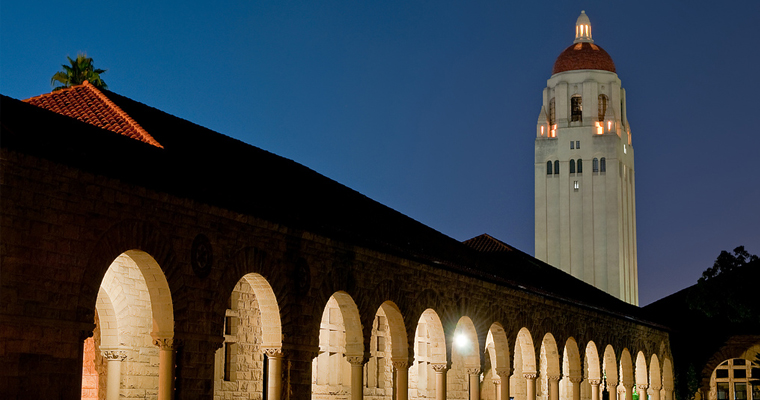
\includegraphics[height=0.20\textheight]{./img/jhonson_content_tower.jpg}\label{fig:tower}}\\ 
      \subfloat[Resultado obtenido transfiriendo el estilo de la obra de arte a la imagen de contenido]
	{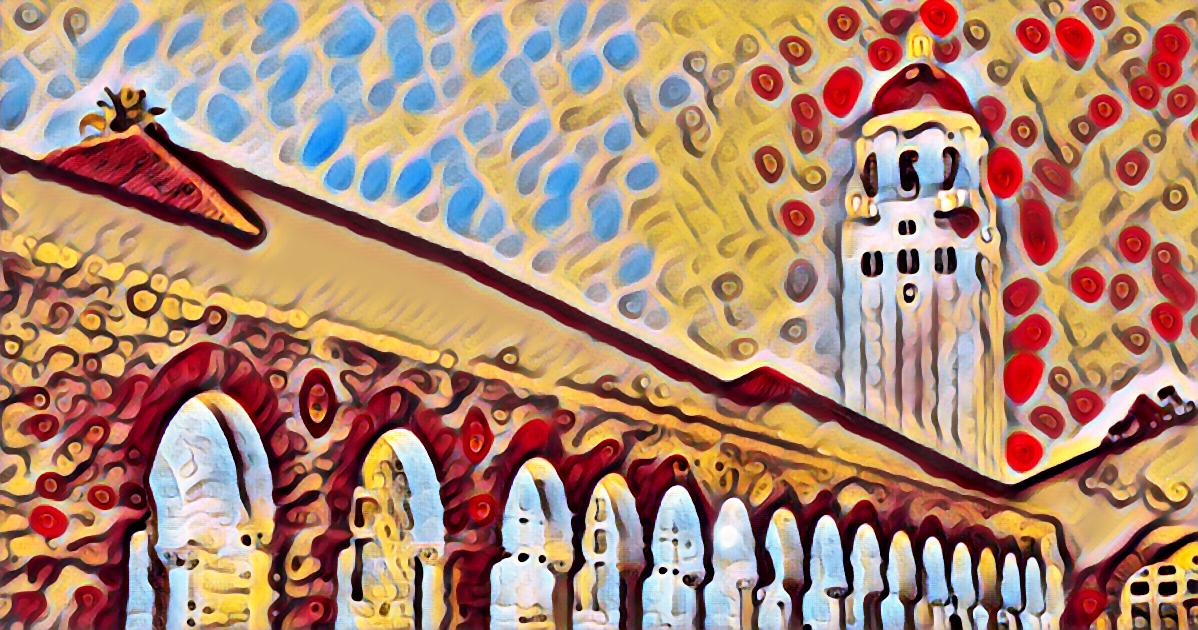
\includegraphics[height=0.20\textheight]{./img/jhonson_result_tower_candy.jpg}\label{fig:candy_tower}}
      
    \end{center}
    \label{fig:style_transfer_candy_tower}
  \end{figure}  
\end{frame}	
  
  
\section{Aprendizaje Automatico}
\begin{frame}
  \frametitle{Aprendizaje Automático}
  Se encuentra en la intersección de las Cs. de la computación y el aprendizaje estadístico 
  Aprendizaje supervisado vs no supervisado: etiquetas
  \begin{figure}[h]
    \begin{center}
      \subfloat[Clasificacion]{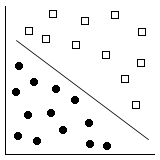
\includegraphics[height=0.20\textheight]{./img/linear_svm.png} \\
      \subfloat[Clustering]{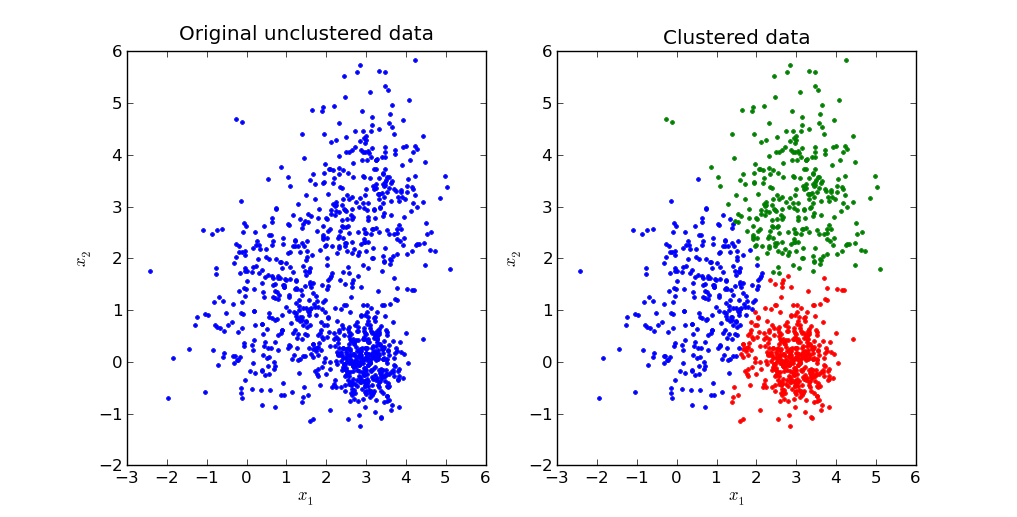
\includegraphics[height=0.20\textheight]{./img/stackoverflow_clustering.png}
    \end{center}
  \end{figure}  
\end{frame}

\begin{frame}
  \frametitle{Clasificacion de imagenes}
  Representacion de la información: Features
  Enfoque clasico vs enfoque aprendizaje profundo
    Enfoque clasico: features predefinidas (Bag of Words) para entrenar el modelo
    Enfoque aprendizaje profundo: Tanto las features como el modelo se entrenan en conjunto
\end{frame}

\begin{frame}
  \frametitle{En que consiste el aprendizaje?}
    Funcion de predicción: mapeo $f_{\theta}: \mathcal{X} {\rightarrow} \{1,\dots,K\}$
    Objetivo del aprendizaje: minimizar $\theta$
    Optimización: minimizar función de pérdida (diferencia entre la predicción y el valor esperado)
\end{frame}

\begin{frame}
  \frametitle{Descenso por el gradiente}
    Optimizar mediante refinamiento iterativo, siguiendo la dirección del gradiente de la función de pérdida.
\end{frame}

\section{Redes Neuronales Artificiales}
\begin{frame}
  \frametitle{Redes Neuronales Artificiales}
    Versión compleja de un clasificador lineal, utilizando funciones no lineales.
    conjunto de unidades de cómputo (neuronas) conectadas en un grafo acı́clico organizadas por capas. 
    Las unidades de una capa se conectan con neuronas de sus capas adyacentes pero nunca se conectan 2 unidades de una misma capa.
    Las funciones 
    \begin{figure}[ht]
      \begin{center}
	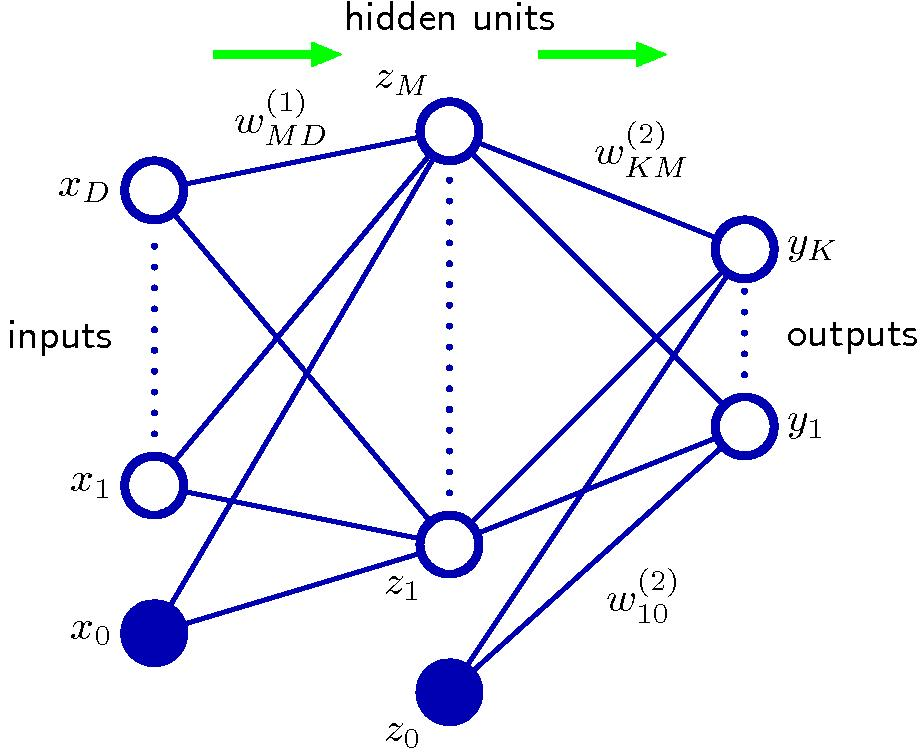
\includegraphics[width=0.8\linewidth]{./img/bishop_neural_network.jpg}
      \end{center}
      \caption{Red Neuronal Artificial}
      \label{fig:neural_network}
    \end{figure}
\end{frame}

\begin{frame}
    \frametitle{Entrenando una red neuronal}
    Ciclos de 2 pasos
    Paso hacia adelante: evaluación de la red en base al dato de entrada
    Retropropagacion: corrección de los pesos internos de la red, según el gradiente de la función de pérdida.
    \begin{figure}[ht]
      \begin{center}
      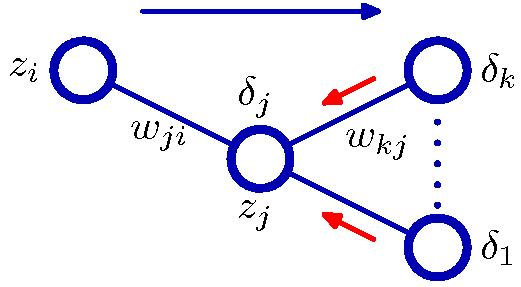
\includegraphics[width=0.5\linewidth]{./img/bishop_backpropagation.jpg}
      \end{center}
      \label{fig:backpropagation}
    \end{figure}
\end{frame}


\section{Redes Neuronales Convolucionales}
\begin{frame}
  \frametitle{Redes Neuronales Convolucionales}
    Redes Neuronales que asumen que sus entradas son imágenes
      Codificar propiedades en la arquitectura de la red:
	Localidad espacial
	Convolucion
	Submuestreo
    
\end{frame}
  
\begin{frame}
  \frametitle{Funcion de convolucion}
    Se aplica un filtro (matriz de 3x3 o 5x5) desplazandolo por toda la imagen.
    Se obtiene una nueva imagen resultante de aplicar el filtro
    \begin{figure}[h]
      \begin{center}
      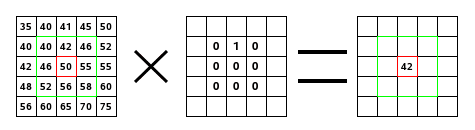
\includegraphics[width=0.8\linewidth]{./img/convolution.png}
      \end{center}
      \caption{Convolución CAMBIAR POR CONVOLUTION WIKI}
      \label{fig:convolution}
    \end{figure}
\end{frame}
  
\begin{frame}
  \frametitle{Estructura de la CNN}
  Capa de Entrada
  Capa de Convolucion
  Capa de Activacion (No lineal)
  Capa de Submuestreo
  Capa de Salida
  \begin{figure}[H]
    \begin{center}
      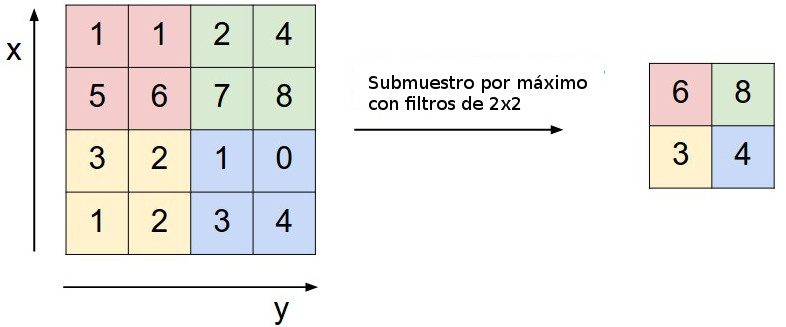
\includegraphics[width=0.8\linewidth]{./img/stanford_maxpool_spanish.jpeg}
    \end{center}
  \end{figure}
      
  \begin{figure}[h]
    \begin{center}
    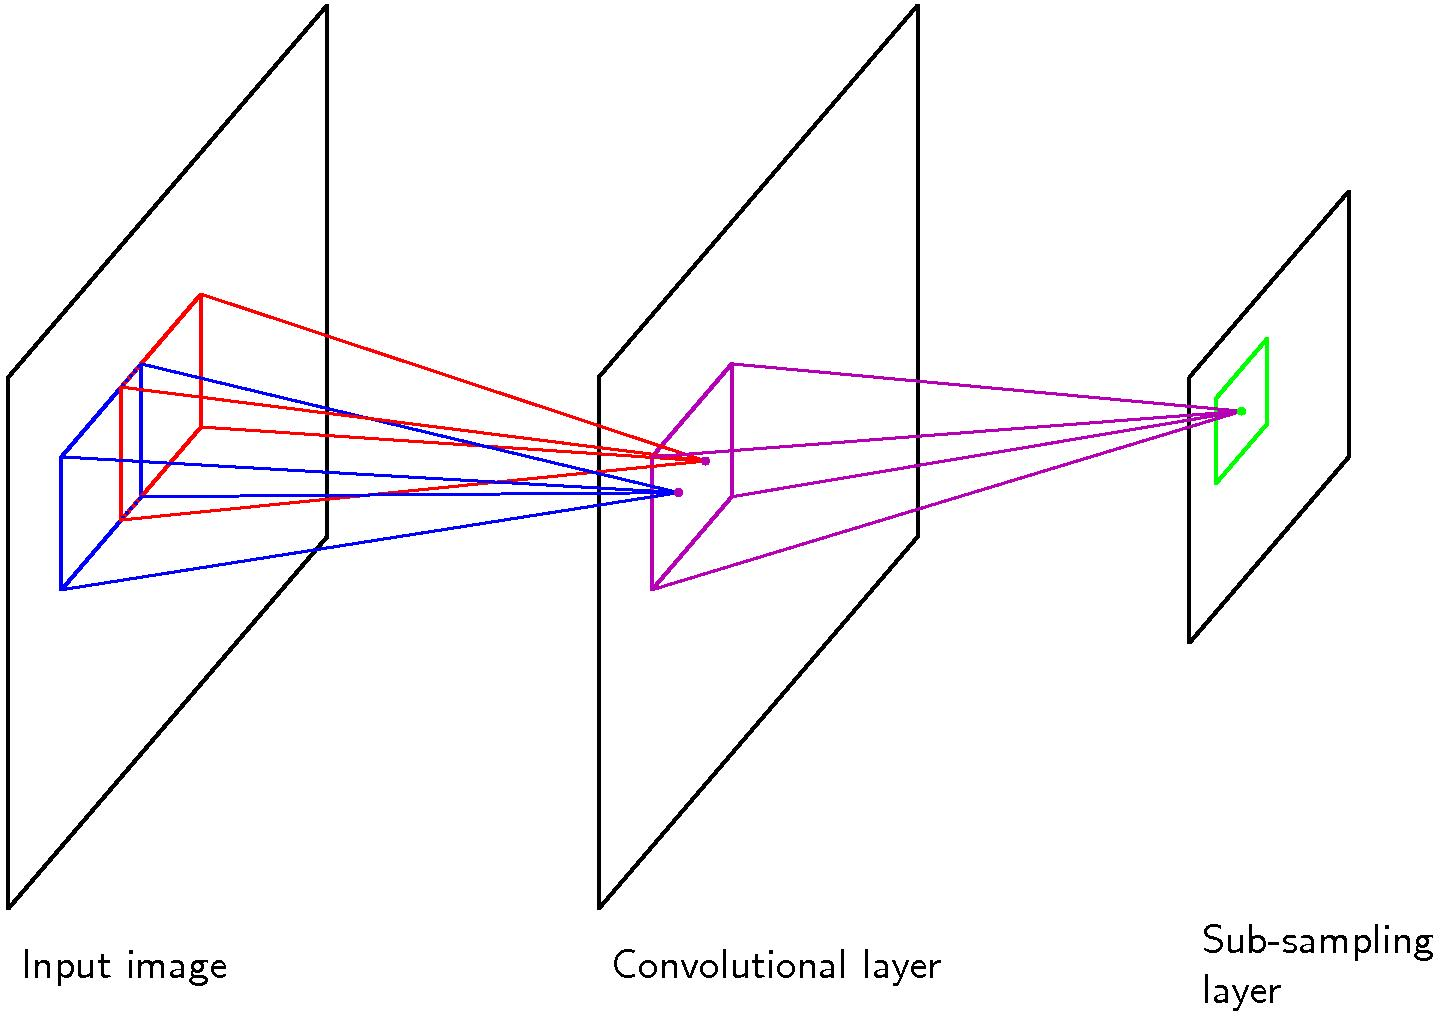
\includegraphics[width=0.8\linewidth]{./img/bishop_cnn.jpg}
    \end{center}
    \caption{Estructura de la CNN}
    \label{fig:convolution}
  \end{figure}
\end{frame}

\section{Ajuste Fino}
\begin{frame}
  \frametitle{Ajuste Fino - Finetuning}
  Adaptar una red preentrenada a un problema similar
  Toma una red preentrenada y un pequeno conjunto de datos
  Reemplaza la ultima capa adaptada al problema
  Reentrena la red comenzando con los pesos predefinidos, ajustandolos a los nuevos datos
\end{frame}


\section{Algoritmo de transferencia de estilo}
\begin{frame}
 \frametitle{Algoritmo de transferencia de estilo}
 Funcion de perdida de estilo
\end{frame}

\begin{frame}
 Funcion de perdida del contenido
\end{frame}

\begin{frame}
 Proceso completo
\end{frame}

\begin{frame}
Hiperparametros
\end{frame}


\section{Elección automática de hiperparámetros}
\begin{frame}
 Descripcion del problema
\end{frame}

\begin{frame}
 Evaluacion
\end{frame}

\begin{frame}
  Solucion propuesta
\end{frame}

\begin{frame}
  Modulo de generacion de imagenes
\end{frame}

\begin{frame}
  Modulo de evaluacion de imagenes
\end{frame}

\section{Experimentos}
\begin{frame}
  \frametitle{Reconocimiento de estilo}
\end{frame}

\begin{frame}
  \frametitle{Imagenes de ejemplo}
\end{frame}

\begin{frame}
  \frametitle{Eleccion del numero de iteraciones}
\end{frame}

\begin{frame}
  \frametitle{Graficos evaluacion vs numero de iteraciones}
\end{frame}

\section{Conclusiones}
\begin{frame}{Conclusiones}
%%%%%%%
\end{frame}



\begin{frame}
 {\Huge ¿Preguntas?}
\end{frame}

\begin{frame}
 {\Huge ¡Gracias por escuchar!}
\end{frame}



% \begin{frame}%%%%%%%%%%
% \frametitle{Referencias}
% \begin{thebibliography}
% 
% %\pause
% \bibitem[KrCla79]{AE-classes}\textrm{Krauss, P.H., Clark, D.M.}, 
% \textit{Global Subdirect Products}, Amer. Math. Soc. Mem. \textbf{210} (1979).
% 
% 
% \end{thebibliography}
% 
% \end{frame}

\begin{frame}
\begin{figure}[center]
% \includegraphics[width=95mm]{19127354.jpg}
%\caption{algebraically closed clones in Post's Lattice} 
\end{figure}
\end{frame}

\end{document}
